\documentclass[aspectratio=1610]{beamer}
\usetheme{Madrid}
% \usepackage{xeCJK}
% \setCJKmainfont{SimSun}
\usepackage{multirow}
\usepackage{graphicx}
\usepackage{booktabs} % for better table formatting
\usepackage{geometry} % for adjusting page layout
\usepackage{hyperref} % for clickable links and references
\usepackage{subcaption}
\usepackage{ctex}
\usepackage{fontspec}
\usepackage{xcolor}
\usepackage{amsmath}
\newtheorem{known}{招聘条件}
% Set fonts with specific shapes and sizes
\setmainfont{SimSun}[
    Scale=1.1
] % Main content font

\setsansfont{Microsoft YaHei}[
    BoldFont={Microsoft YaHei Bold},
    ItalicFont={Microsoft YaHei Light},
    BoldItalicFont={Microsoft YaHei Bold},
    Scale=1.2
] % Sans-serif font, often used for titles

\setmonofont{FangSong}[
    Scale=1.2
] % Monospaced font

% Customize Beamer theme to use these fonts
\setbeamerfont{title}{family=\sffamily,series=\bfseries,size=\huge} % Title font to sans-serif, bold, and large
\setbeamerfont{frametitle}{family=\sffamily,series=\bfseries,size=\Large} % Frame title font to sans-serif, bold, and large
\setbeamerfont{normal text}{family=\rmfamily,series=\mdseries,size=\normalsize} % Normal text font to serif
\setbeamerfont{author}{family=\rmfamily,series=\itshape,size=\large}

\title{量子软件工程师\\面试}
\author{高丁超}
\date{\today}

\begin{document}

\frame{\titlepage}
\section{个人简介}
\begin{frame}
\frametitle{个人信息}
\begin{itemize}
    \item 出生年份:2000.01
    \item 教育经历: 
    \begin{itemize}
        \item \textbf{2017-2021},西安电子科技大学,学士
        \item \textbf{2021-2024},中科院软件研究所,硕士
    \end{itemize}
    \item 邮件地址:by.gdc@outlook.com
    \item Github: https://github.com/gcc-bug
\end{itemize}
\end{frame}

\section{项目经历}
\begin{frame}
\frametitle{项目简介}
\begin{enumerate}
    \item \textbf{张量决策图项目} 
    \begin{itemize}
        \item 使用python完善基于张量决策图的工具
        \item 使用C++ 重构张量决策图工具,并设计python接口
    \end{itemize}
    \item \textbf{线性可逆量子电路综合}*,\textit{2024},用C++实现线性可逆量子电路综合
    \item \textbf{量子密码项目},\textit{2024},调研并部分实现simon和量子随机游走在密码领域的应用
    \item \(\dots\)
\end{enumerate}
\end{frame}

\begin{frame}
\frametitle{张量决策图}
\begin{figure}
    \centering
    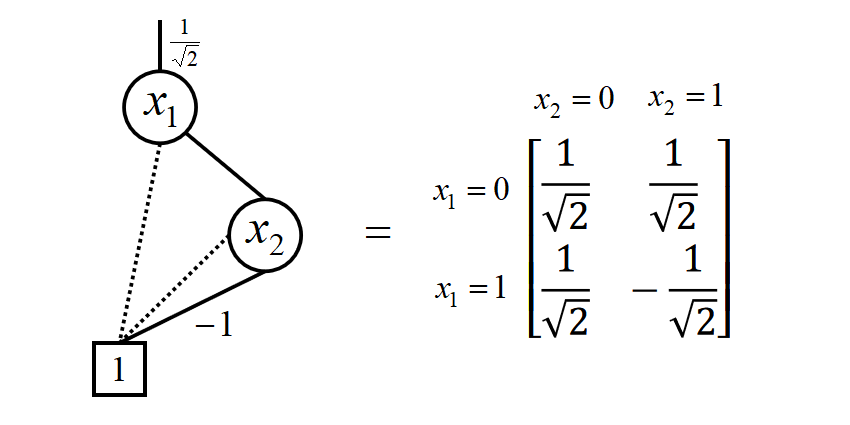
\includegraphics[height=6cm]{TDD_H_gate2.png}
    \caption{张量决策图提供了更紧凑的表示量子操作的方式}
\end{figure}
\end{frame}
\begin{frame}
\frametitle{张量决策图项目}
\begin{figure}[htbp]
    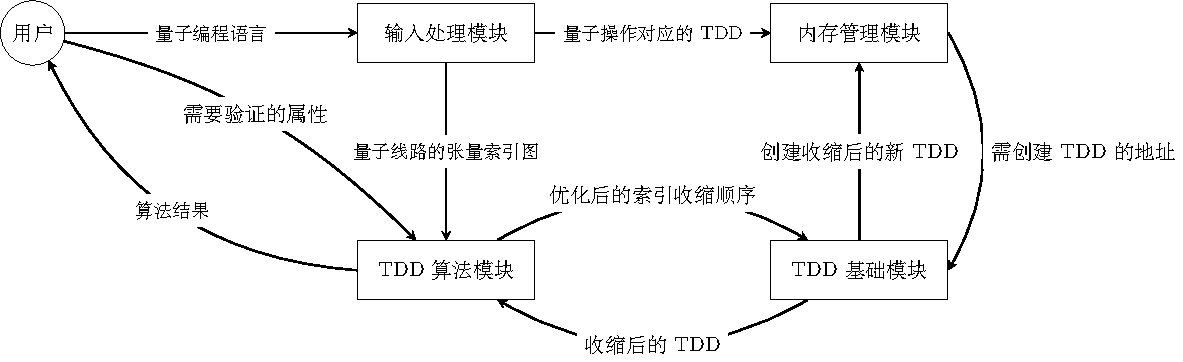
\includegraphics[width=\textwidth]{alg_flow.pdf}
    \caption{软件模块之间的调用关系}
    \label{fig-flow}
\end{figure}
\end{frame}

\begin{frame}
\frametitle{编程技能}
\begin{itemize}
    \item python, c++, c-python 混合编程
    \item xtensor, qiskit, numpy等软件包
    \item cmake, pybind11 架构
\end{itemize}
\end{frame}

\begin{frame}
    \frametitle{电路综合项目}
    \begin{figure}[ht]
        \centering
        \begin{subfigure}{0.45\textwidth}
            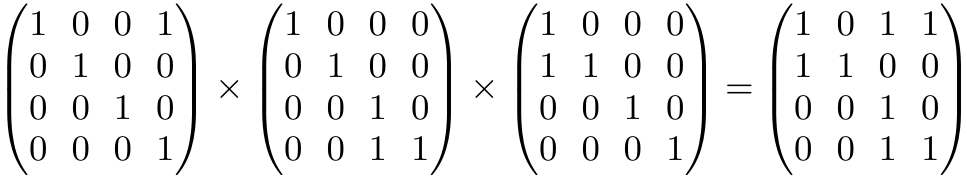
\includegraphics[width=1.2\linewidth]{cnot.png}
        \end{subfigure}
        \hfill
        \begin{subfigure}{0.45\textwidth}
            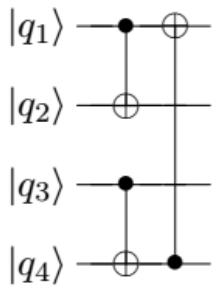
\includegraphics[width=.5\linewidth]{cnot_circuit.png}
        \end{subfigure}
        \caption{线性可逆电路可以用矩阵的行列变换表示}
        \label{fig:figures}
    \end{figure}
\end{frame}
\begin{frame}
    \frametitle{电路综合项目}
    \begin{figure}[htbp]
        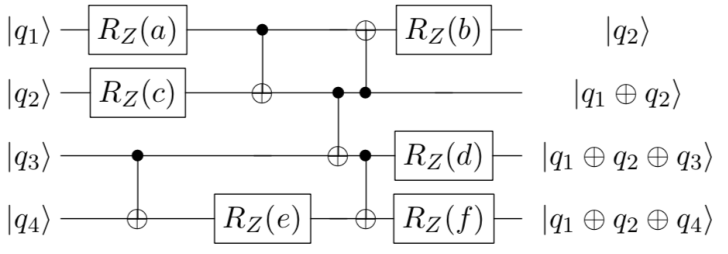
\includegraphics[width=.8\textwidth]{phase.png}
        \caption{可以进一步推广线路可逆电路综合方法到phase network电路}
    \end{figure}
\end{frame}
\begin{frame}
    \frametitle{电路综合项目}
    \begin{figure}[htbp]
        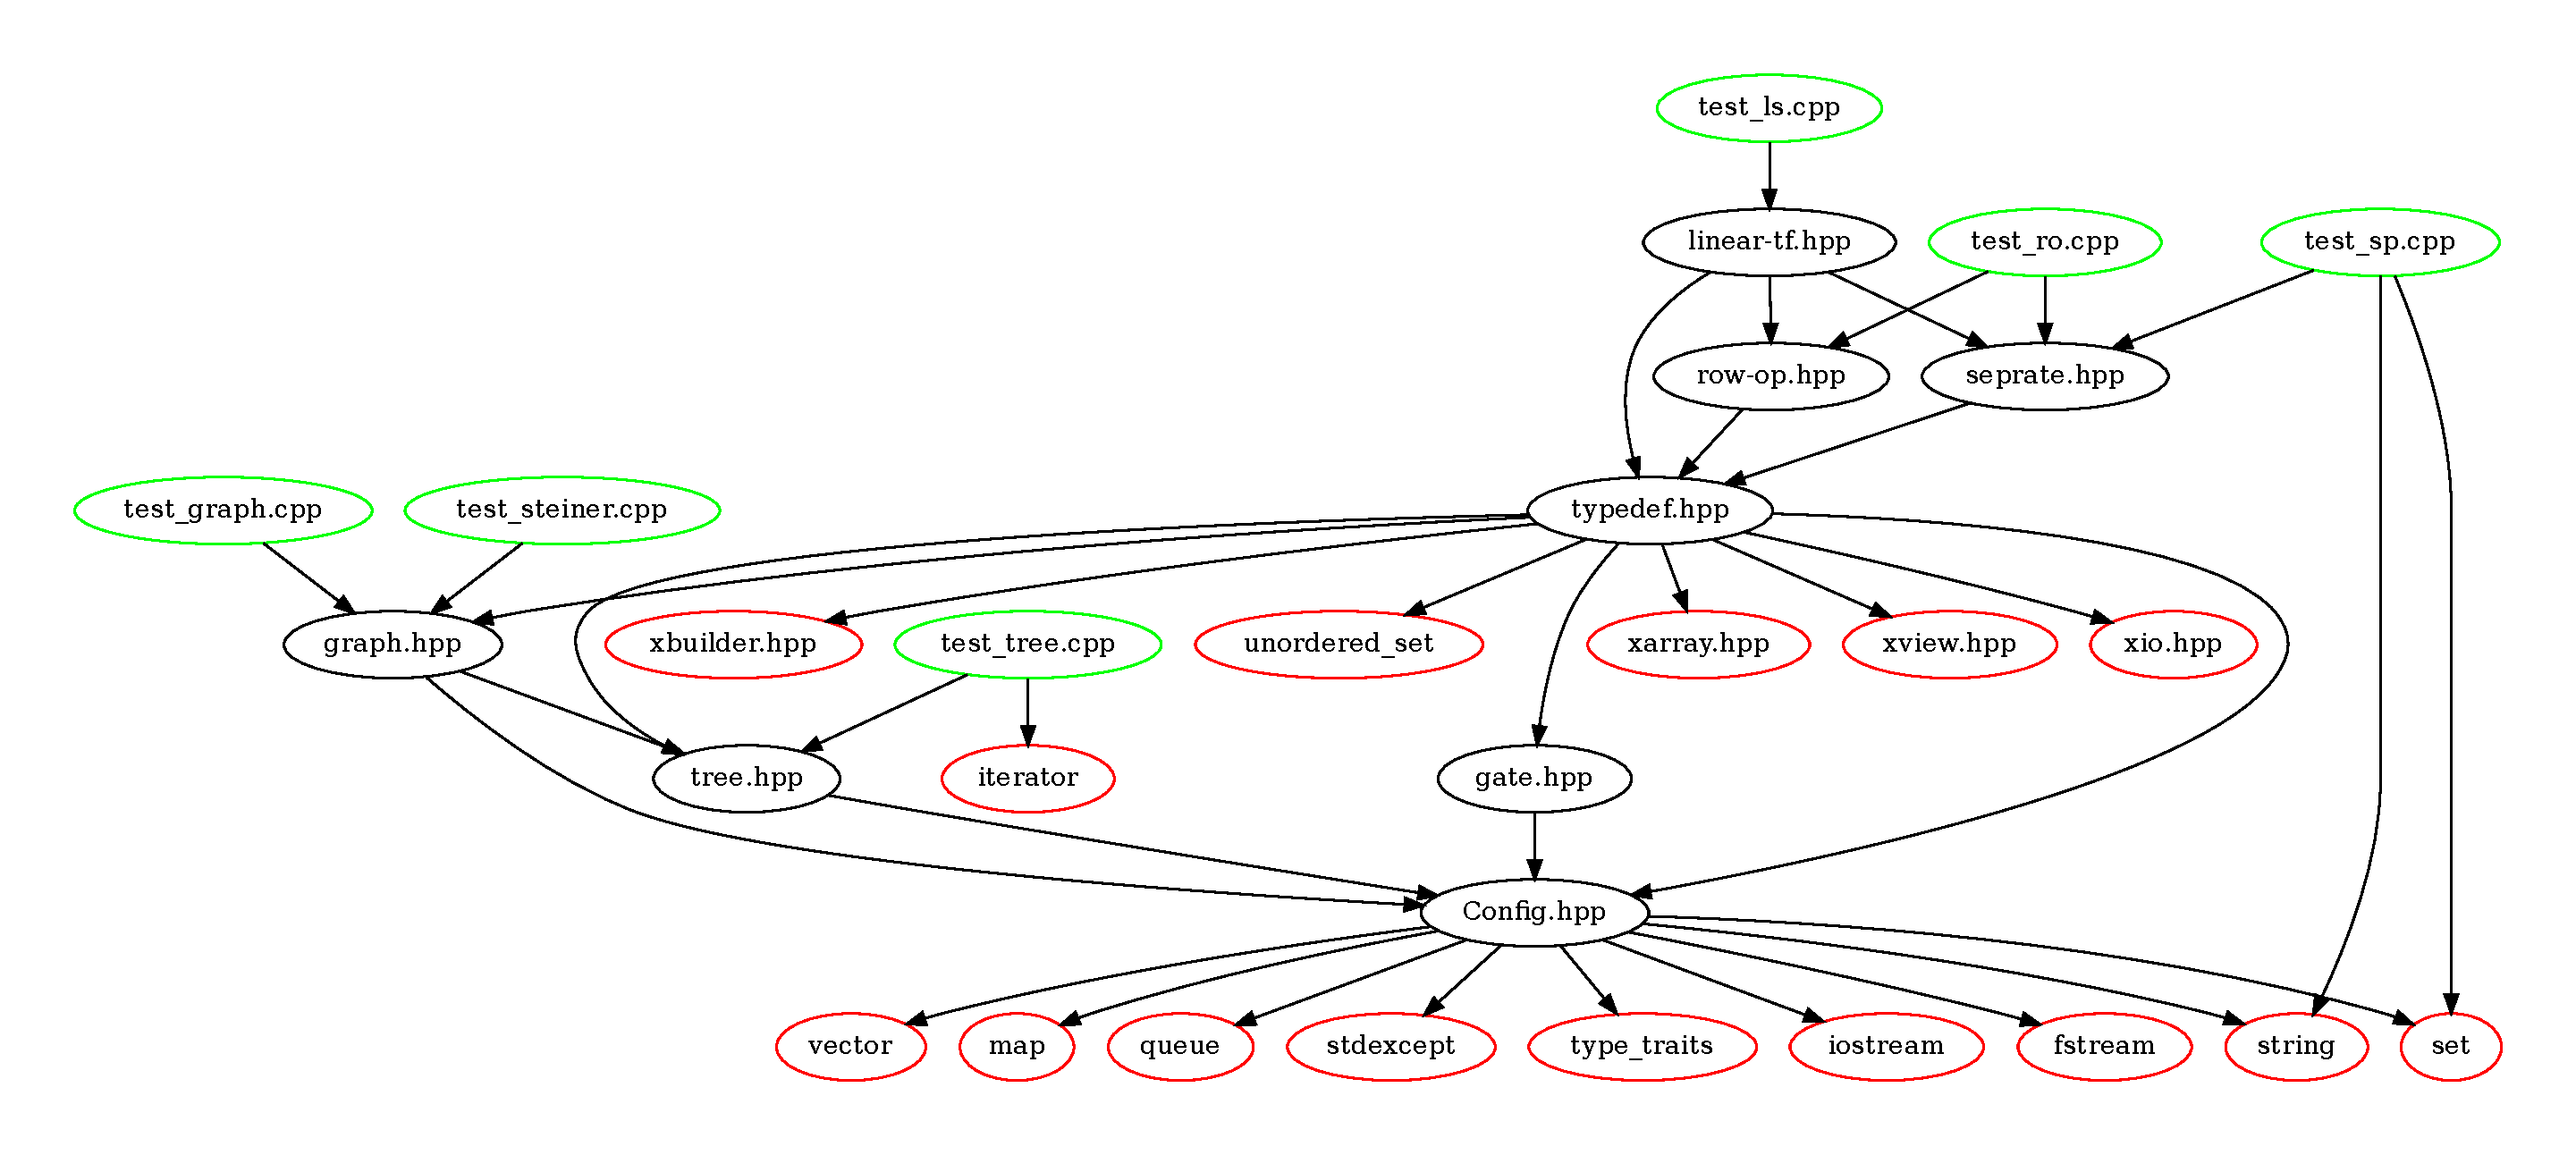
\includegraphics[width=.8\textwidth]{dep.pdf}
        \caption{项目内容}
    \end{figure}
\end{frame}
\begin{frame}
    \frametitle{密码项目-simon}
    \begin{figure}[htbp]
        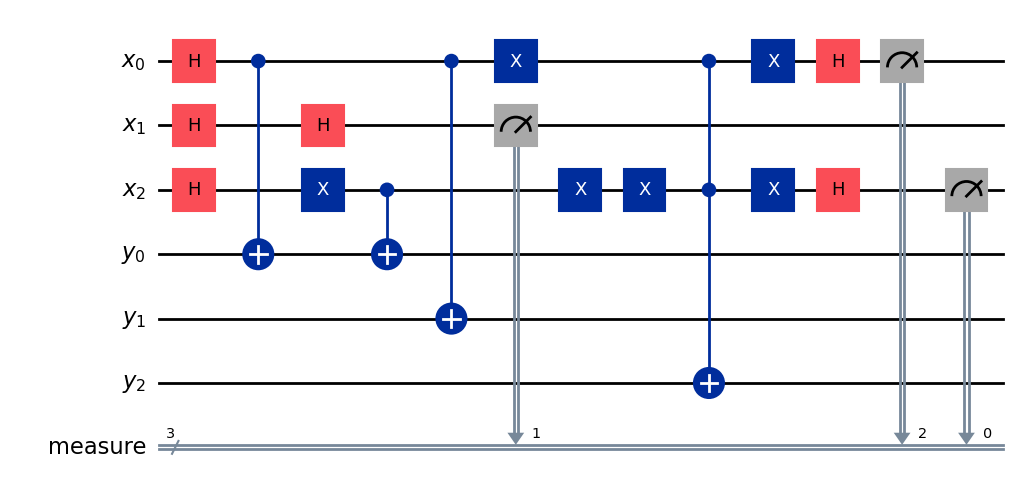
\includegraphics[width=.8\textwidth]{simon.png}
        \caption{项目内容}
    \end{figure}
\end{frame}

\begin{frame}
    \frametitle{密码项目-量子随机游走}
    \begin{figure}[htbp]
        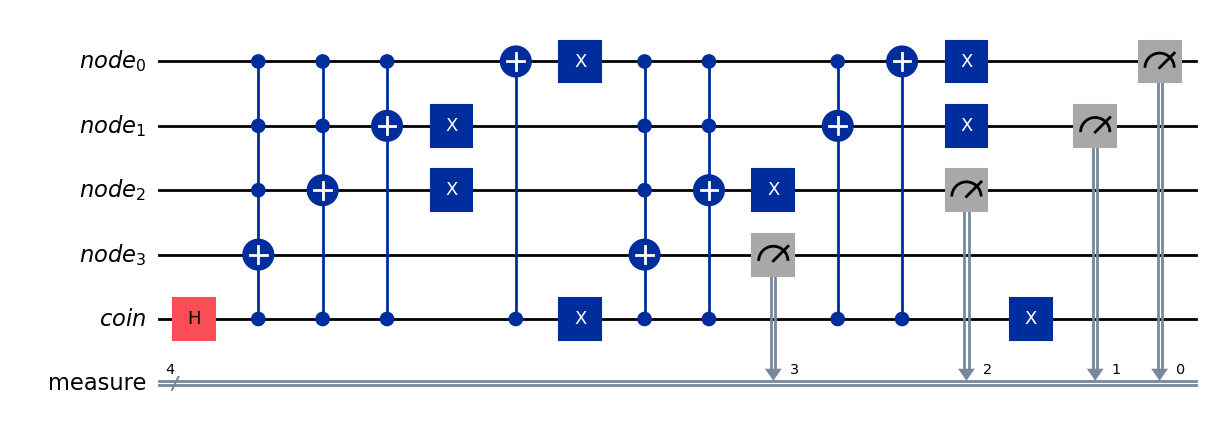
\includegraphics[width=.8\textwidth]{qw.png}
        \caption{项目内容}
    \end{figure}
\end{frame}

% \begin{frame}
% \frametitle{Achievements and Recognition}
% \begin{itemize}
%     \item Award 1: [Description]
%     \item Recognition 1: [Description]
% \end{itemize}
% \end{frame}

\begin{frame}
\frametitle{其他项目与技能}
\begin{itemize}
    \item \textbf{VQE项目},用isq-python实现氢分子基态能量的计算
    \item \textbf{VHDL},实现过STM32架构下蓝牙模块与传感器的通信
    \item \textbf{COQ},完成过Softwarefoundation中卷一的逻辑命题的证明
\end{itemize}
\end{frame}

\begin{frame}
\frametitle{Q\&A}
\begin{center}
    Any Questions?
\end{center}
\end{frame}

\end{document}
